\documentclass[10pt]{scrartcl}

\usepackage{fullpage}
\usepackage{amsmath}
\usepackage{amsthm}
\usepackage{url}
\usepackage{relsize}
\usepackage{xspace}
\usepackage{subfigure}
\usepackage{graphicx,color}
\usepackage{amssymb}
\usepackage[margin=0.82in]{geometry}

\def\TODO#1{\noindent\textbf{[TODO: #1}]}

\begin{document}
\title{Predicting the Stock Market with Newspaper Articles}
\subtitle{6.867 Final Project}
\author{Chris Johnson \and Fredrik Kjolstad}
\date{December 10, 2012}
\maketitle

\begin{abstract}

\end{abstract}

\section{Introduction}

\section{Data and Feature Selection}

Our data set consists of 36,466 Wall Street Journal (WSJ) articles over 359 days, and 251 days of closing price information of the Dow Jones Industrial Average (DJI) for the year 2007. The stock market is closed on weekends and holidays, which is why there are fewer days of stock data than newspaper articles. There are two days for which we have stock data but no newspaper articles (December 18th and 27th), but this appears to be an omission in the provided data set. We consider only days for which we have both WSJ and DJI data. 

We have approximately 101 articles per day on average. A histogram of articles per day appears in Figure~\ref{articlehist}. The distribution appears to be bimodal, with numbers of articles around either 125 or 15 per day. Since some days have fewer articles, which may decrease their effectiveness for classification. 

\TODO{Maybe we want to scale counts per day, but for NB this doesn't matter. Maybe some of the dimensionality reduction techniques are returning which days have more articles!}

\begin{figure}
\centering
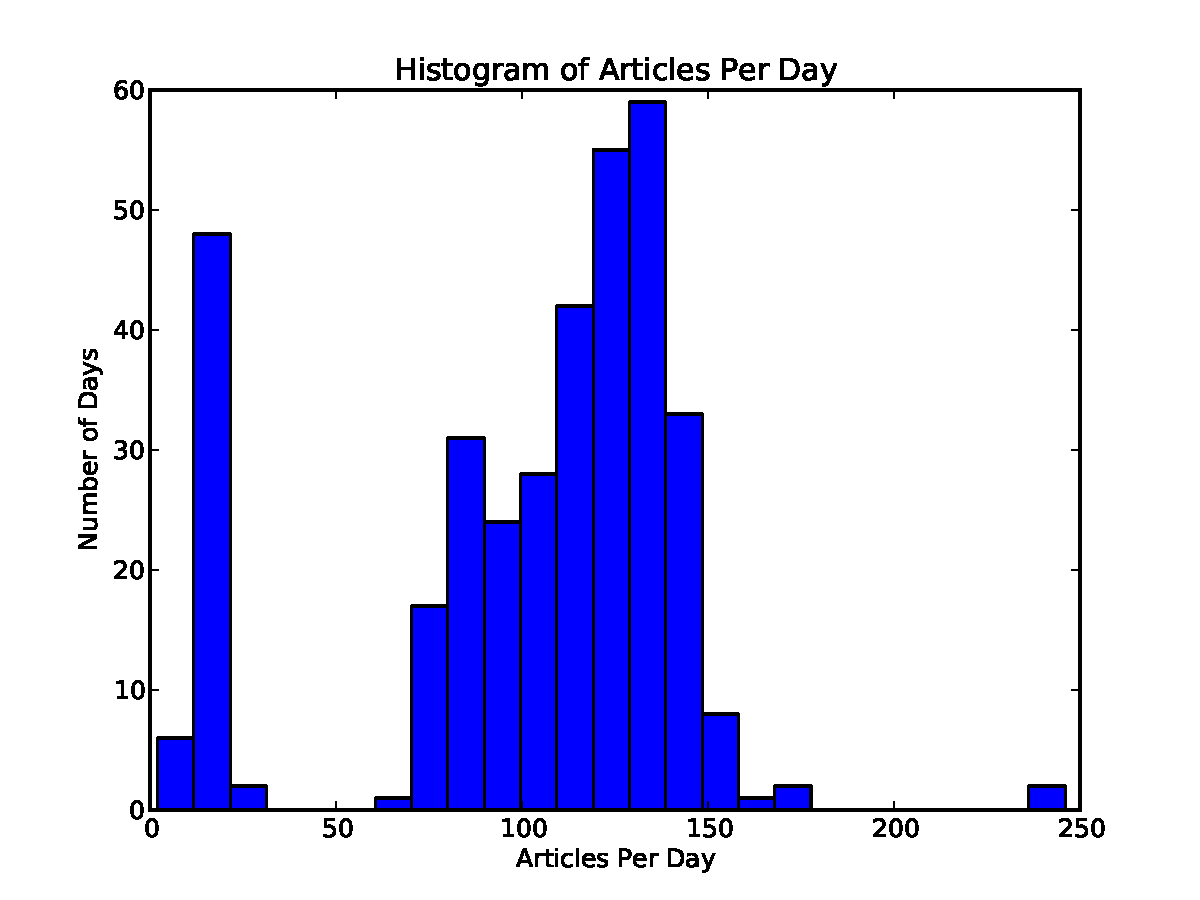
\includegraphics[scale=0.3]{text/articleshist.pdf}
\caption{Histogram of Articles Per Day}

\label{articlehist}
\end{figure}

Our data set consists of over 24 million words, with an average of 667 words per article. A histogram of article lengths appears in Figure~\ref{wordshist}. Most articles tend to be less than 2000 words, but there appears to be a long tail consisting of a few very long articles. For the most part it appears that article lengths are similar apart from a few outliers.


\begin{figure}
\centering
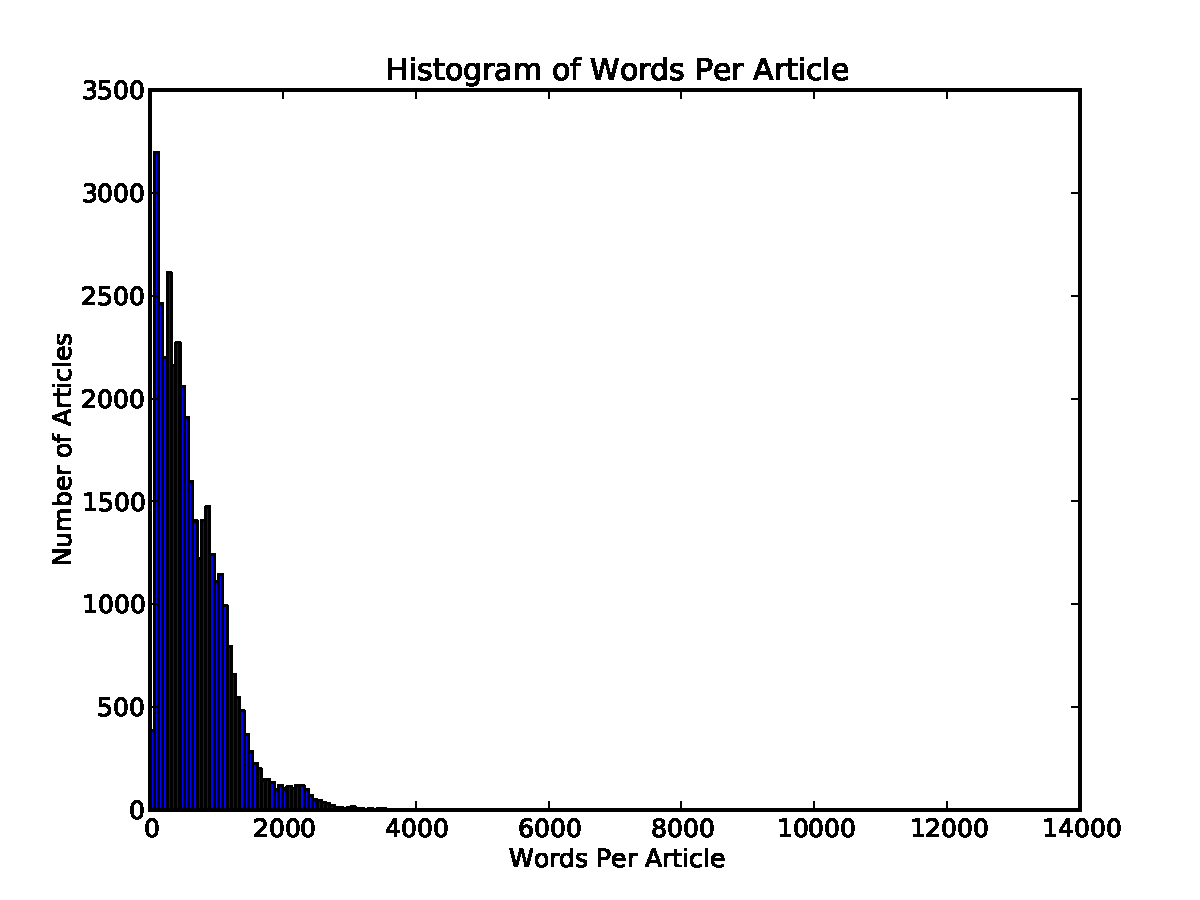
\includegraphics[scale=0.3]{text/wordshist.pdf}
\caption{Histogram of Words Per Article}
\label{wordshist}
\end{figure}

The data set contains 150,875 unique words. Each data point we use for training and validation therefore consists of a class label (+1 if the market went up that day, -1 if it went down) and a feature vector computed using frequencies of these unique words.

Due to the difficulty of computation on the number of unique words that we have, we filtered out any words that did not appear more than some cutoff, $m$, throughout the year. We assume that these words are either misspellings or words which would not generally be useful in predicting stock performance due to their infrequency. Filtering with $m = 10$ results in 44,218 unique words and was found to be a good balance between information and computationbal tractability.
Additionally, we filtered out any of the 100 most commonly used English words~\footnote{http://en.wikipedia.org/wiki/Most\_common\_words\_in\_English}, since we
assume that words such as ``and'' and ``I'' do not provide very much information out of context.

The rest of this section describes several feature extraction techniques that we used with the machine learning algorithms presented in Section~\ref{sec:techniques}, and we describe the form of the resulting feature vectors.

Terminology \TODO{introduce this right}:

$F_{d,i}$ the ith element of the feature vector for day $d$.

$W$ the set of all words

$A$ the set of all articles (each of which is a set of words frequencies)

$D$ the set of days, each of which is a set of articles

\paragraph{Bag of Words}

The simplest feature vector is simply a ``bag of words'' for each day~\cite{featurehash}, which consists of frequency counts of all words in any article on that day. Elements of the feature vector take the form: $$\displaystyle F_{d,i} = \sum_{A \in D_d}{A_i}$$ These feature vectors are extremely sparse, since most articles do not use tens of thousands of unique words (we represent our data set as a sparse matrix
in MATLAB to reduce memory consumption to reasonable levels).

\TODO{Read the paper that is cited and see if implementing hashing is good, seems our assumptions are different from theirs}

\TODO{Exhaustively discuss all feature selections here and cite sources}

\TODO{Read all sources and be familiar with them for interview!}
 

\section{Techniques}
\label{sec:techniques}

\section{Evaluation}
\begin{itemize}
\item The word ``ambitions'' is the best indicator of the Dow Jones gaining. If ``ambitions'' appeared in the WSJ there was a 64.26\% chance that the Dow Jones went up on that day.
\item The word ``tundra'' is the best indicator of the Dow Jones falling. If ``tundra'' appeared in the WSJ there was a 64.26\% chance that the Dow Jones fell on that day. This is because a series of articles in the WSJ where they talk about how Toyota is producing more cars outside the us and where they mention the Toyota Tundra.
\end{itemize}

\bibliographystyle{plain}
\bibliography{report.bib}

\end{document}
